\documentclass{article}
\usepackage[T1]{fontenc}
\usepackage{lmodern}
\usepackage{graphicx}
\usepackage{amsmath,amssymb}
\usepackage[a4paper,margin=2cm]{geometry}
\usepackage[absolute,overlay]{textpos}
\setlength{\TPHorizModule}{1mm}
\setlength{\TPVertModule}{1mm}
\usepackage[indonesian]{babel}
\usepackage{hyperref}
\setlength{\emergencystretch}{2em}
% unit: Halaman 40

\begin{document}

% === Halaman 40 (llm) ===

\begin{itemize}
  \item Dari Gambar tersebut dapat dilihat bahwa:

\vspace{115.83mm}

  \begin{align*}
    C_i &= P_i \oplus E_k(C_{i-1}) \\
    P_i &= C_i \oplus D_k(C_{i-1})
  \end{align*}

  yang dalam hal ini, $C_0 = IV$.

  \vspace{20mm}

  \item Kesalahan 1-bit pada suatu blok plainteks tertentu akan merambat pada blok cipherteks yang berkoresponden dan blok-blok cipherteks selanjutnya pada proses enkripsi.
\end{itemize}

% deskripsi: Diagram alir proses enkripsi Cipher Block Chaining (CBC) yang menunjukkan penggunaan IV, blok plainteks P, fungsi enkripsi Ek, dan hasil cipherteks C.
% bbox normalisasi: [0.4400, 0.1900, 0.9700, 0.5800]
\begin{textblock*}{111.30mm}(92.40mm,56.43mm)
\noindent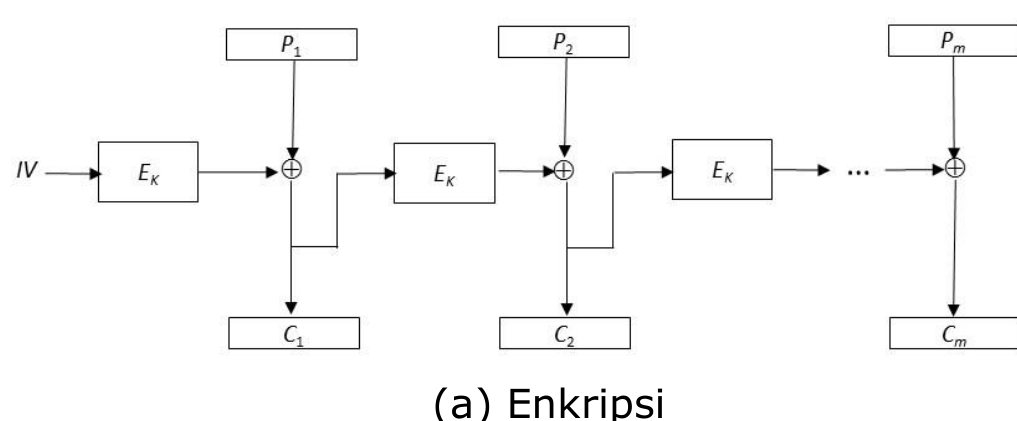
\includegraphics[width=111.30mm,height=115.83mm]{../../images/llm/page_040_img_01.png}%
\end{textblock*}

\end{document}
